\chapter{Interpolation of Simplified Model dark matter limits}
\label{app:interpolation}

In order to fully populate the $m_{med}$-$m_{DM}$ plane, more parameter points than reasonably available as FullSim MC samples are necessary.
To this end, a reweighting of the available FullSim samples is performed.

Terminology used in this section:
\begin{itemize}
\item \textbf{FullSim samples}: The samples we get from central production with proper detector simulation. We have 38 (28) of these for the axial (vector) mediators.
\item \textbf{Target}: a parameter point/sample we want to obtain using our reweighting technique.
\item \textbf{Reference}: The parameter point/sample we use as a basis to get to the target. The reference is always one of the FullSim samples.
\end{itemize}

\section{Calculating the weights}
Using the same \MADGRAPH model as used for central production, generator-level spectra of the mediator transverse momentum $\pt^{med}$ are obtained.
While in the centrally produced samples, \MADGRAPH is used to calculate jet multiplicities of both zero and one,the generator samples only contain the zero jet process from \MADGRAPH. 
This is due to the practical limitation that processing time increases dramatically with an added jet, which makes it impossible to
generate a larger number of parameter points for reweighting in this configuration. However, it is found that simply using the 0 jet samples alone is sufficient for the reweighting.

To mimic the effects of the analysis selection, a generator-level selection is applied before extracting the $\pt^{med}$ spectra.

\begin{itemize}
\item $\pt^{\rm lepton} > 20 \GeV.             $
\item $|\eta^{\rm lepton}| < 2.5               $
\item $\pt^{ll} > 60 \GeV                      $
\item $\Delta\phi(ll,med) > 2.6                $
\item $|\pt^{ll} - \pt^{\rm med} / \pt^{\rm med}| < 0.4$
\item $\Delta R (ll) < 1.8$
\end{itemize}

The $\pt^{med}$ distributions are scaled according to the generated cross-section before applying the additional selection criteria.
This ensures that differences in acceptance between target and reference are taken into account.

For a given target and reference, the ratio of the $\pt^{med}$ distributions is then used as a $\pt^{med}$-dependent weight.

$$ w(\pt^{med}) = \frac{P^{\rm target}(\pt^{med}) }{ P^{\rm reference}(\pt^{med})}$$

Where $w$ is the weight and $P(\pt^{med})$ is the value of the $\pt^{med}$ distribution at a given value of $\pt^{med}$.


\section{Choosing a reference}
For a given target point, a reference sample is chosen by minimizing the distance between reference and target in the $log(m_{med})$-$log(m_{DM})$ plane.
In order to improve the performance of the procedure, the optimization is constrained to only allow the reference sample to have relatively larger
DM mass than the target  $m_{DM}^{target} / m_{med}^{target}  \leq m_{DM}^{ref} / m_{med}^{ref}$. This requirement aims to take
into account that the shape of the \MET spectrum becomes increasingly harder as $m_{DM}$ increases.


\section{Closure testing}
In order to test this method, it is possible to reweight FullSim samples to represent parameter points that are also available in FullSim.
Thus, one may compare the ``real'' and reweighted final \MET distribution and check their agreement.
It has to be noted that this method will generally give a worst-case impression of the performance of the reweighting.
Since one reweights FullSim to FullSim, the average distance between target and reference will be much larger than in the
real use case, where one always reweights to the nearest FullSim sample.

For each reweighted FullSim sample, the bin-by-bin difference between real and reweighted bin content divided by its statistical uncertainty is recorded
(\textit{bin-by-bin pull}). In the absence of systematical shifts induced by the method, the pulls should scatter around zero with a standard deviation of one.
The distributions for axial and vector mediators are shown in fig.~\ref{fig:app_interp_pulls}. Only target points with $100\GeV < m_{med} < 2000\GeV$ are considered.
In both cases, the width of the distribution is consistent with unity no significant bias in the mean is observed.

The distribution of the pulls is also given per target parameter point (fig.~\ref{fig:app_interp_pulls_per_point}) and as a function of \MET (fig.~\ref{fig:app_interp_pulls_2d}). These views allow to see in more detail the behavior of the reweighting and spot possibly pathological features that could be obscured in the overall distributions. No systematic trends are found, indicating that the method works sufficiently well. This assessment has of course to be taken relative to the attainable precision in this test: Due to the limited signal sample statistics, the precision of the closure test method is limited and it is not necessary to obtain a perfect interpolation method, since the limited-statistics argument applies also to the actual analysis case.

A closure test of the expected limits is shown in fig.~\ref{fig:app_interp_mu_pulls}, showing good agreement in the final median expected limit, which ultimately determines the Z value in the 2D scan.  Good agreement is observed.


%-----------------------------------------------------
 \begin{figure}[htbp]
   \begin{center}
	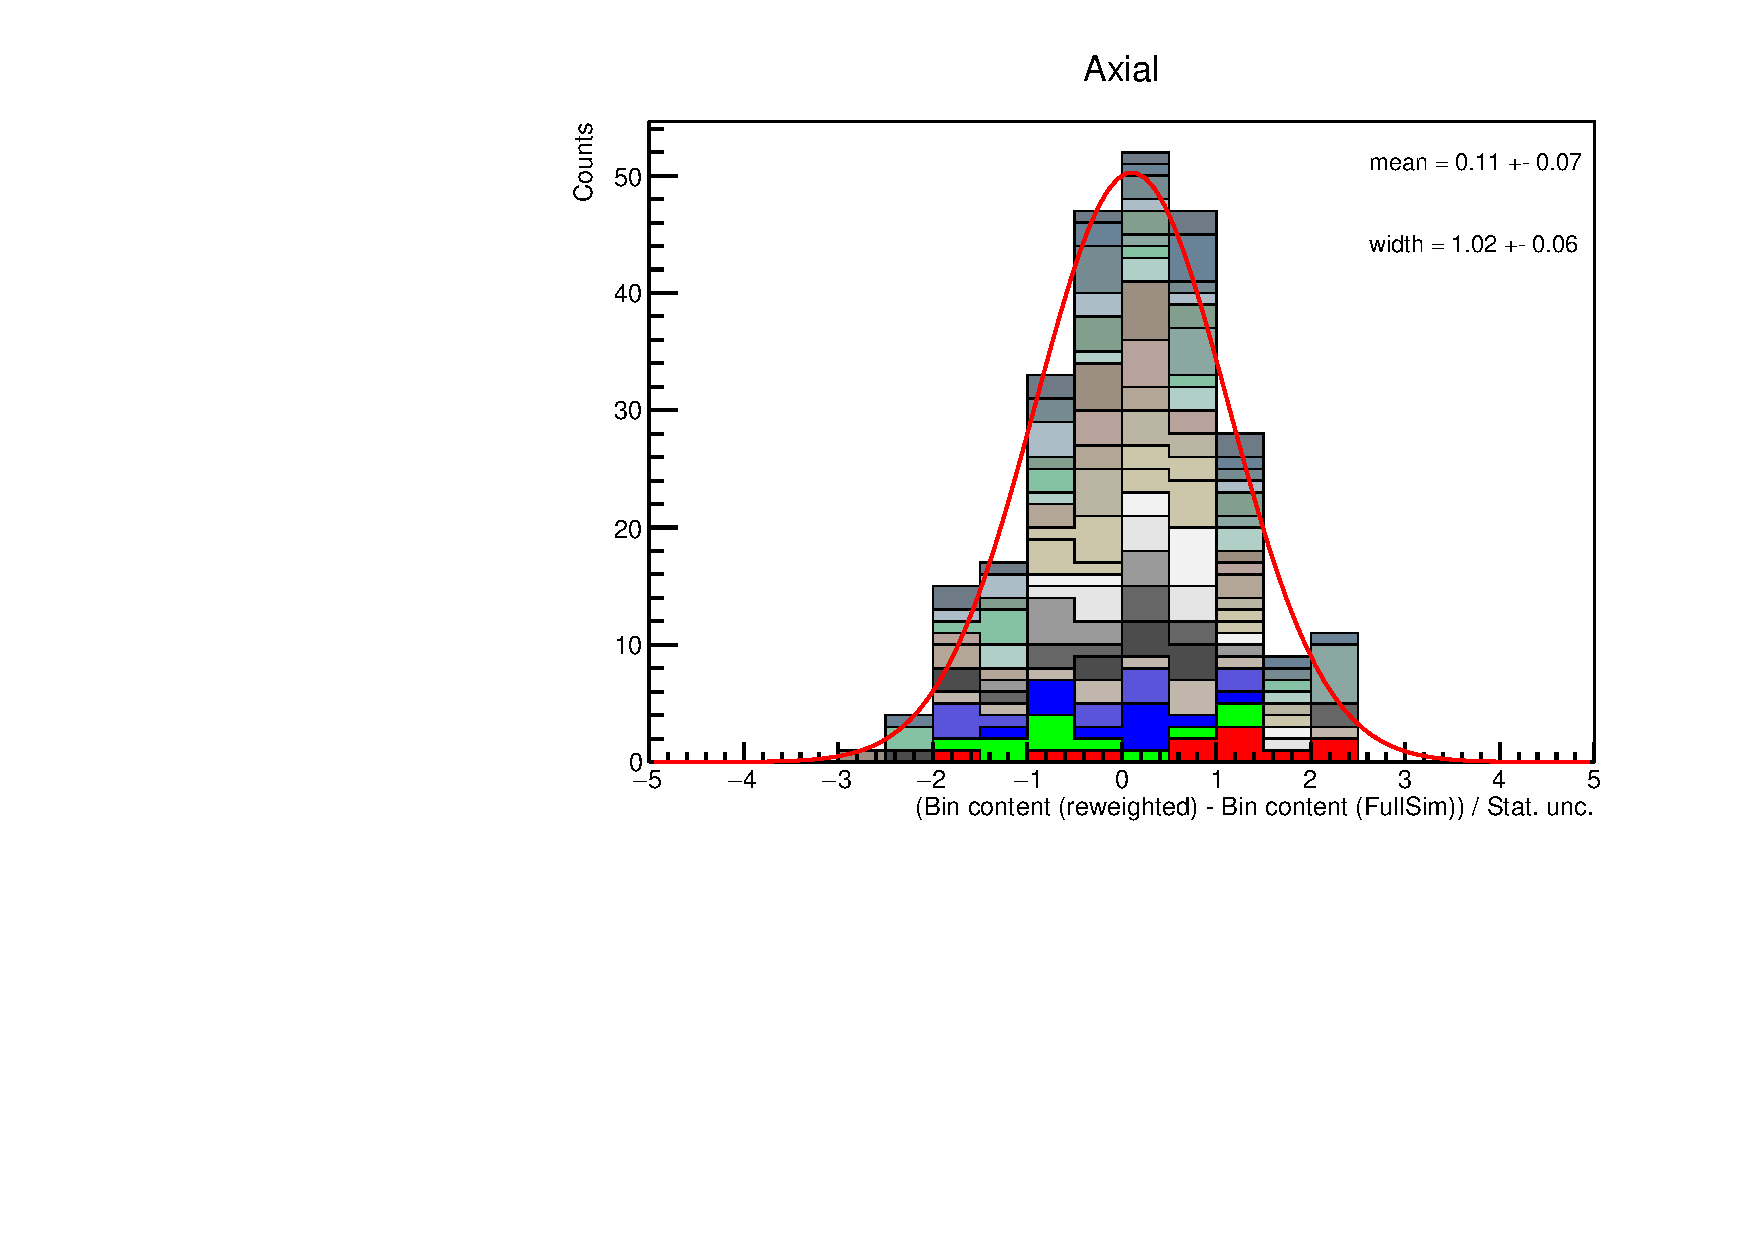
\includegraphics[width=0.45\textwidth]{figures/interpolation_appendix/Axial_pulls.pdf}
	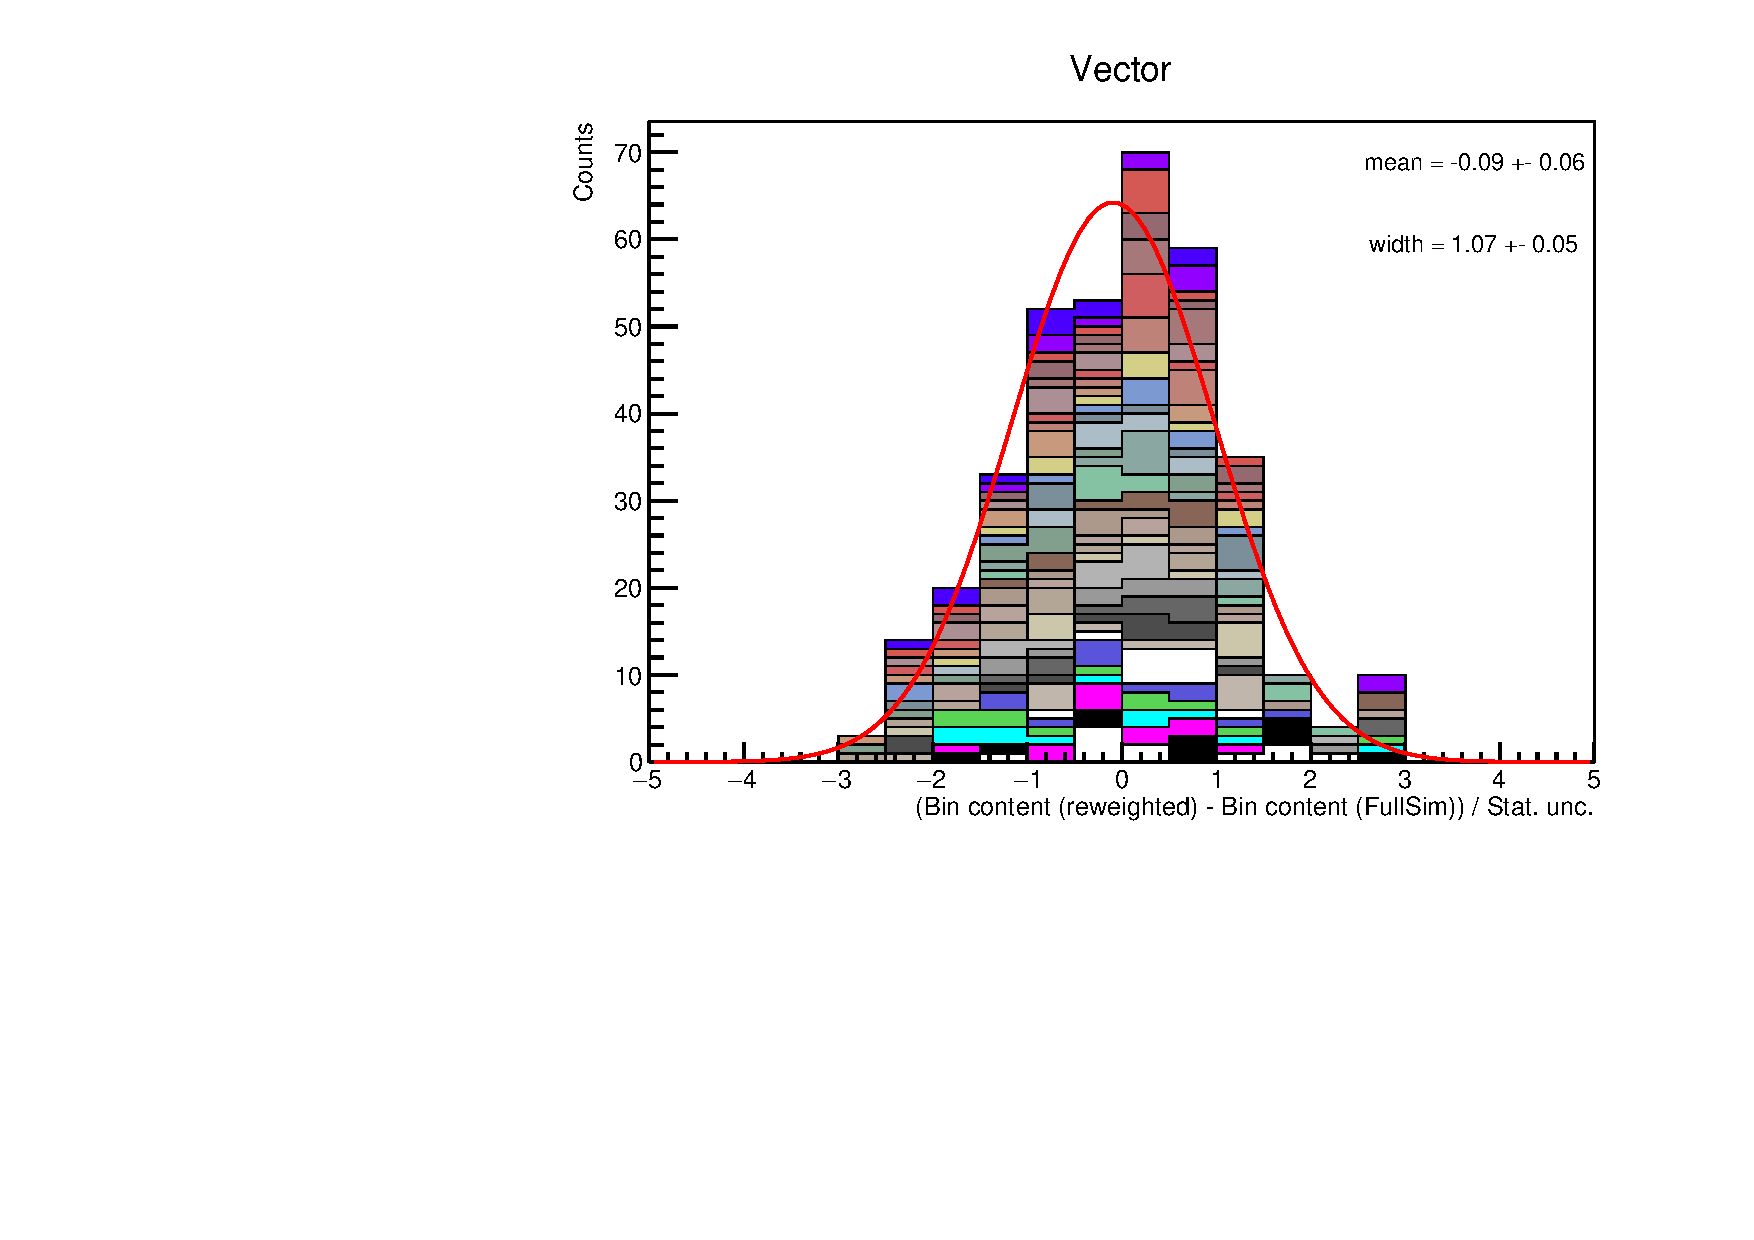
\includegraphics[width=0.45\textwidth]{figures/interpolation_appendix/Vector_pulls.pdf}
     \caption{Bin-by-bin pull distribution in the axial (left) and vector mediator cases (right).
				For details on how these pulls are calculated, refer to the text. Each color represents one target sample
				(If the colors are confusing to, you may ignore them altogether, in which case you will see the overall distribution in all points).}
     \label{fig:app_interp_pulls}
   \end{center}
 \end{figure}
 %-----------------------------------------------------

%-----------------------------------------------------
 \begin{figure}[htbp]
   \begin{center}
	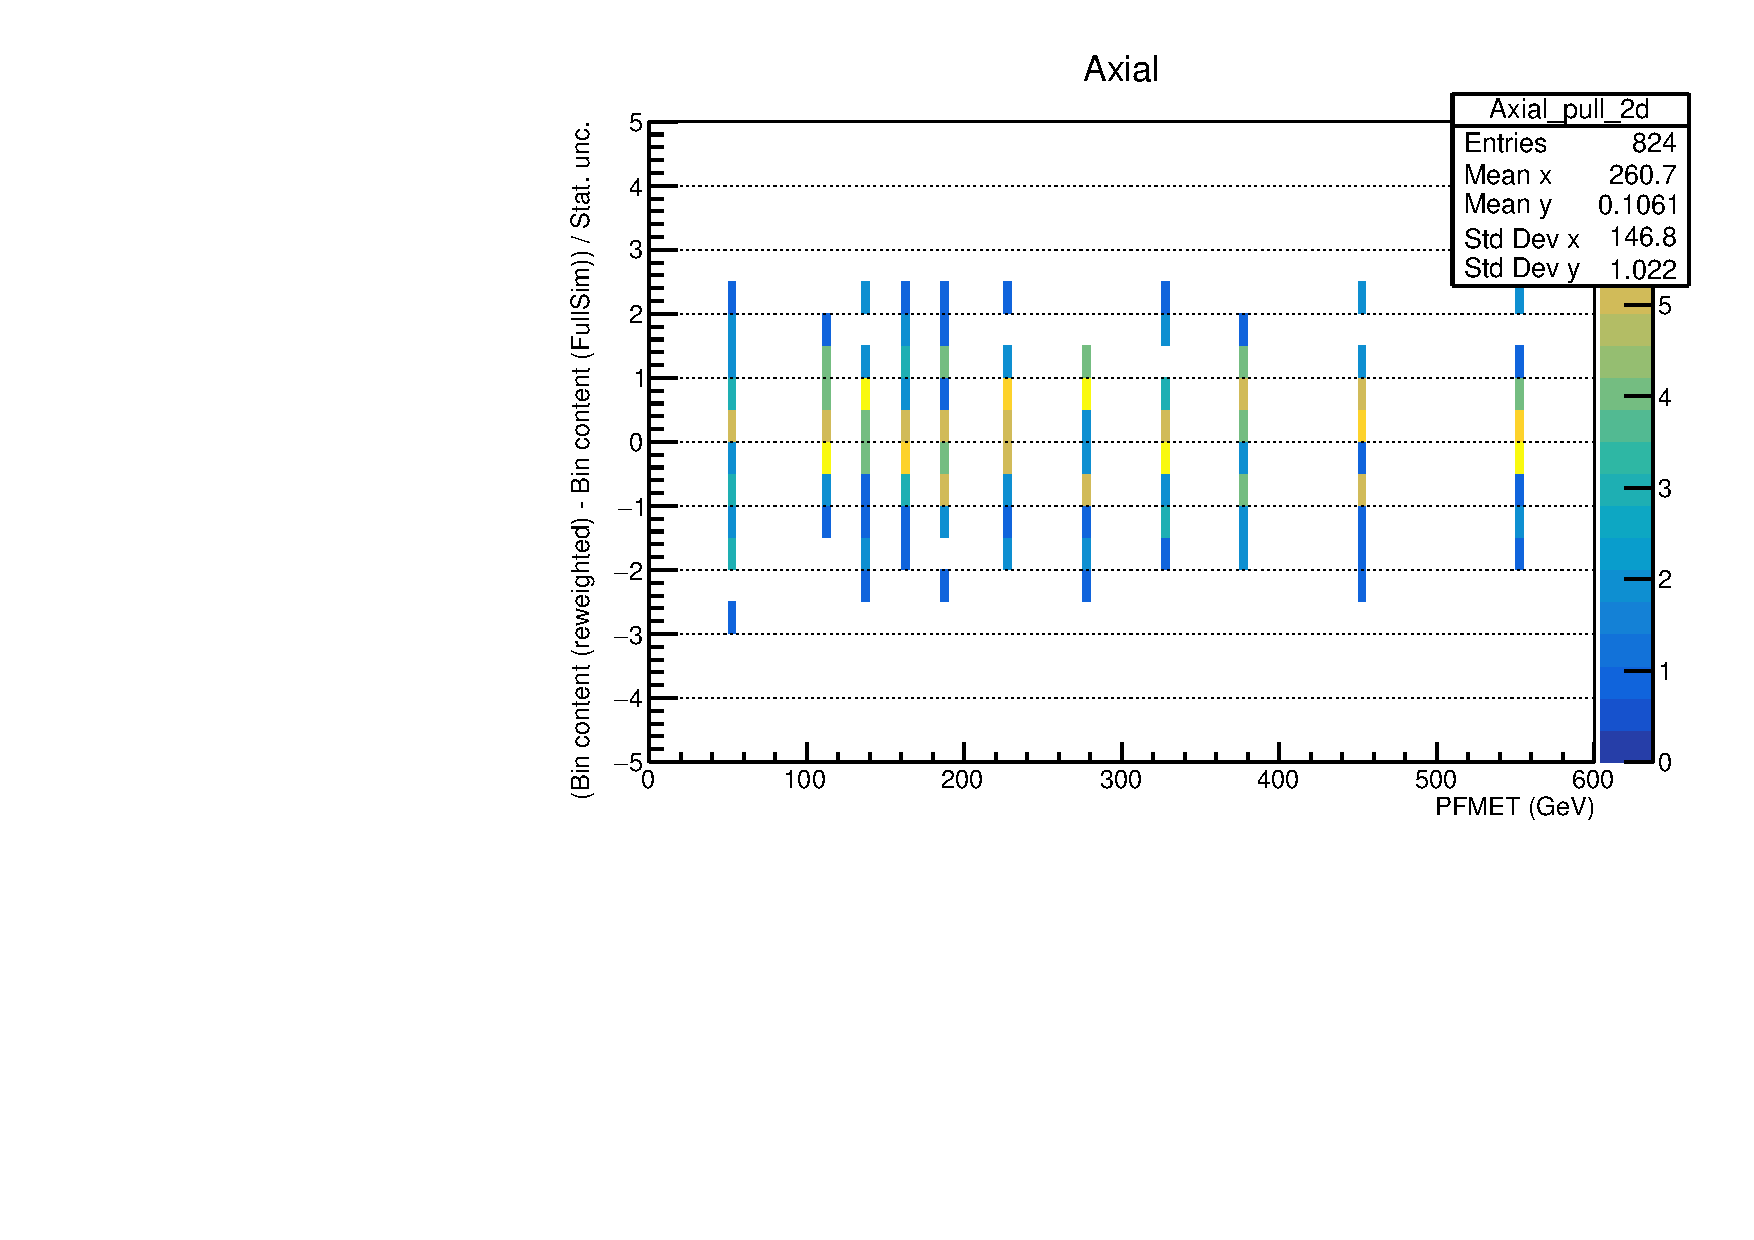
\includegraphics[width=0.45\textwidth]{figures/interpolation_appendix/Axial_pulls_2d.pdf}
	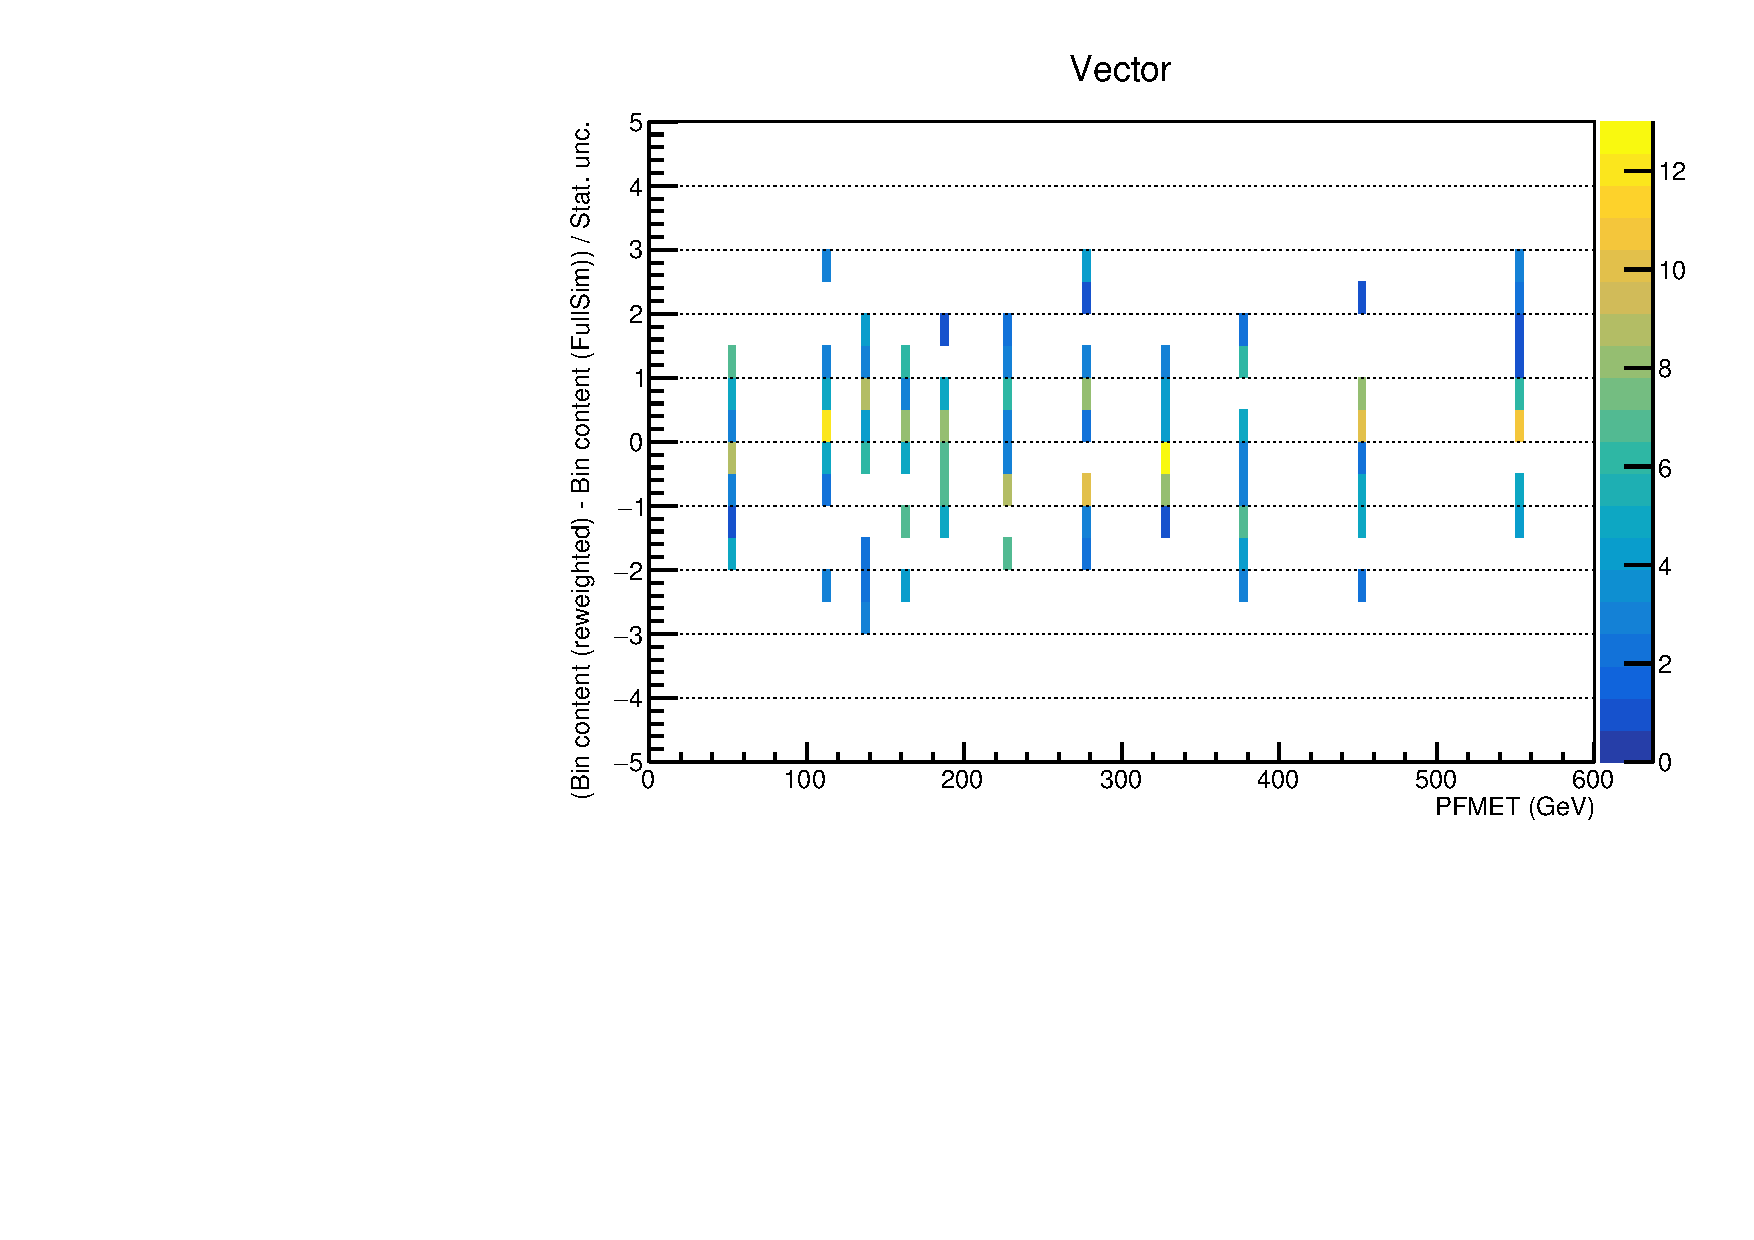
\includegraphics[width=0.45\textwidth]{figures/interpolation_appendix/Vector_pulls_2d.pdf}
     \caption{Same as fig.~\ref{fig:app_interp_pulls}, but the pull distributions are shown as a function of PFMET.}
     \label{fig:app_interp_pulls_2d}
   \end{center}
 \end{figure}
 %-----------------------------------------------------

%-----------------------------------------------------
 \begin{figure}[htbp]
   \begin{center}
	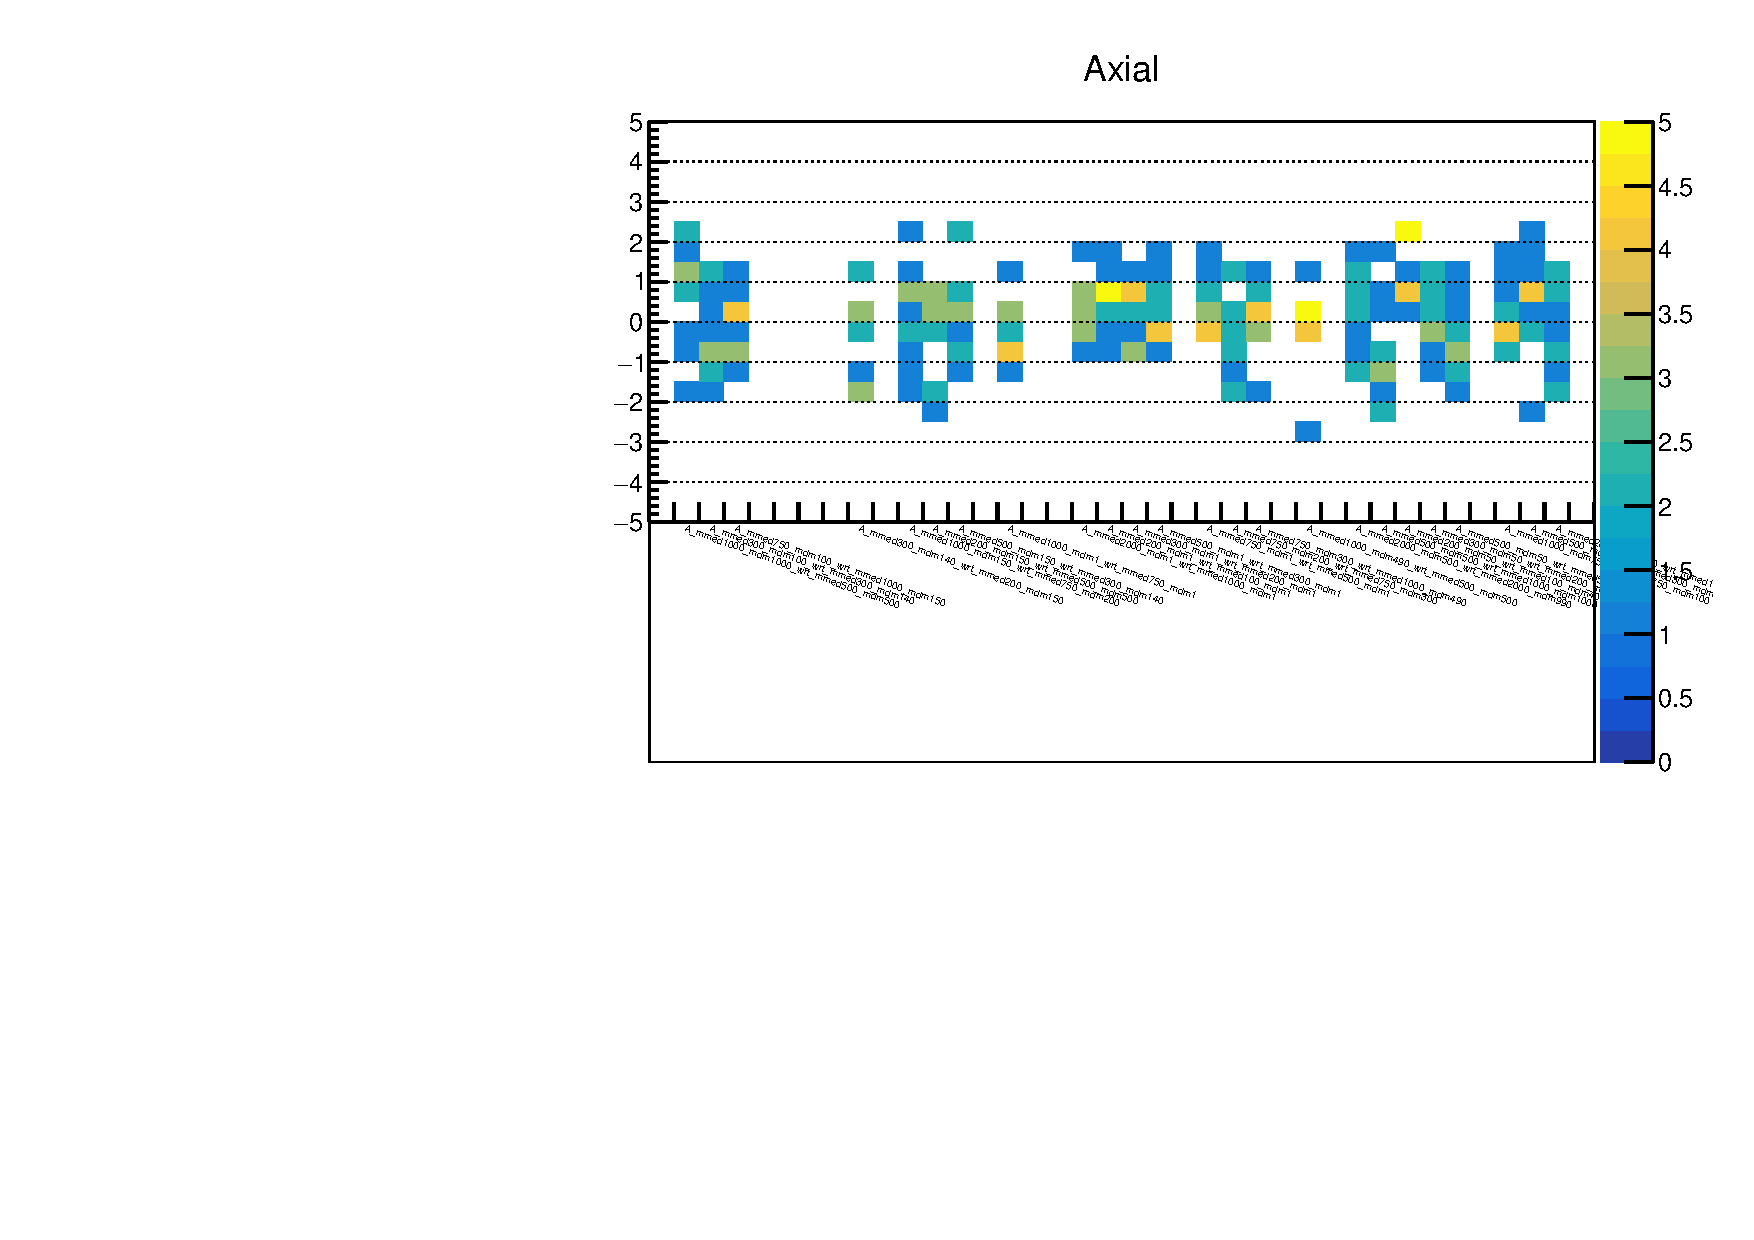
\includegraphics[width=0.9\textwidth]{figures/interpolation_appendix/Axial_pulls_per_point.pdf}
	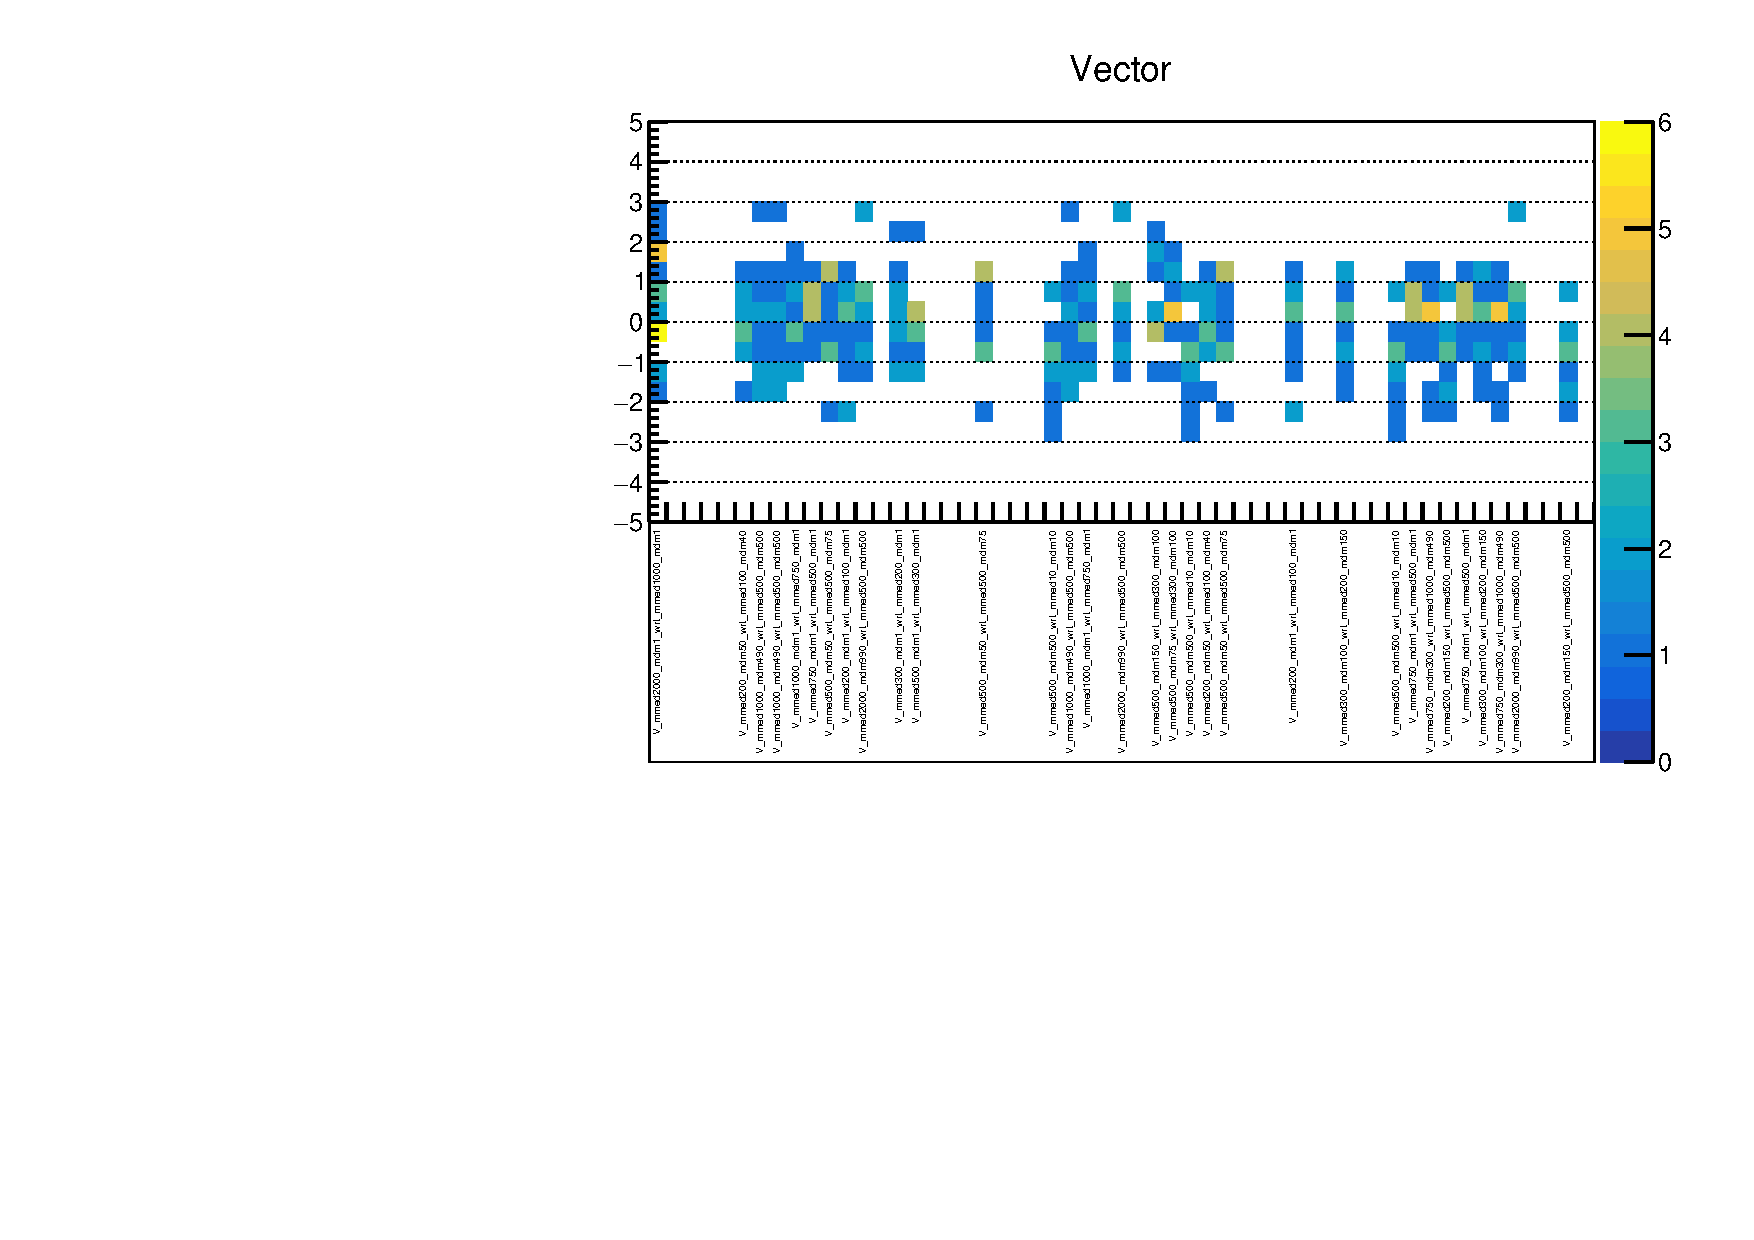
\includegraphics[width=0.9\textwidth]{figures/interpolation_appendix/Vector_pulls_per_point.pdf}
     \caption{Same as fig.~\ref{fig:app_interp_pulls}, but the pull distributions are shown for each individual target point. Each vertical bin in this view corresponds to one color in fig.~\ref{fig:app_interp_pulls}.}
     \label{fig:app_interp_pulls_per_point}
   \end{center}
 \end{figure}
 %-----------------------------------------------------

%-----------------------------------------------------
 \begin{figure}[htbp]
   \begin{center}
	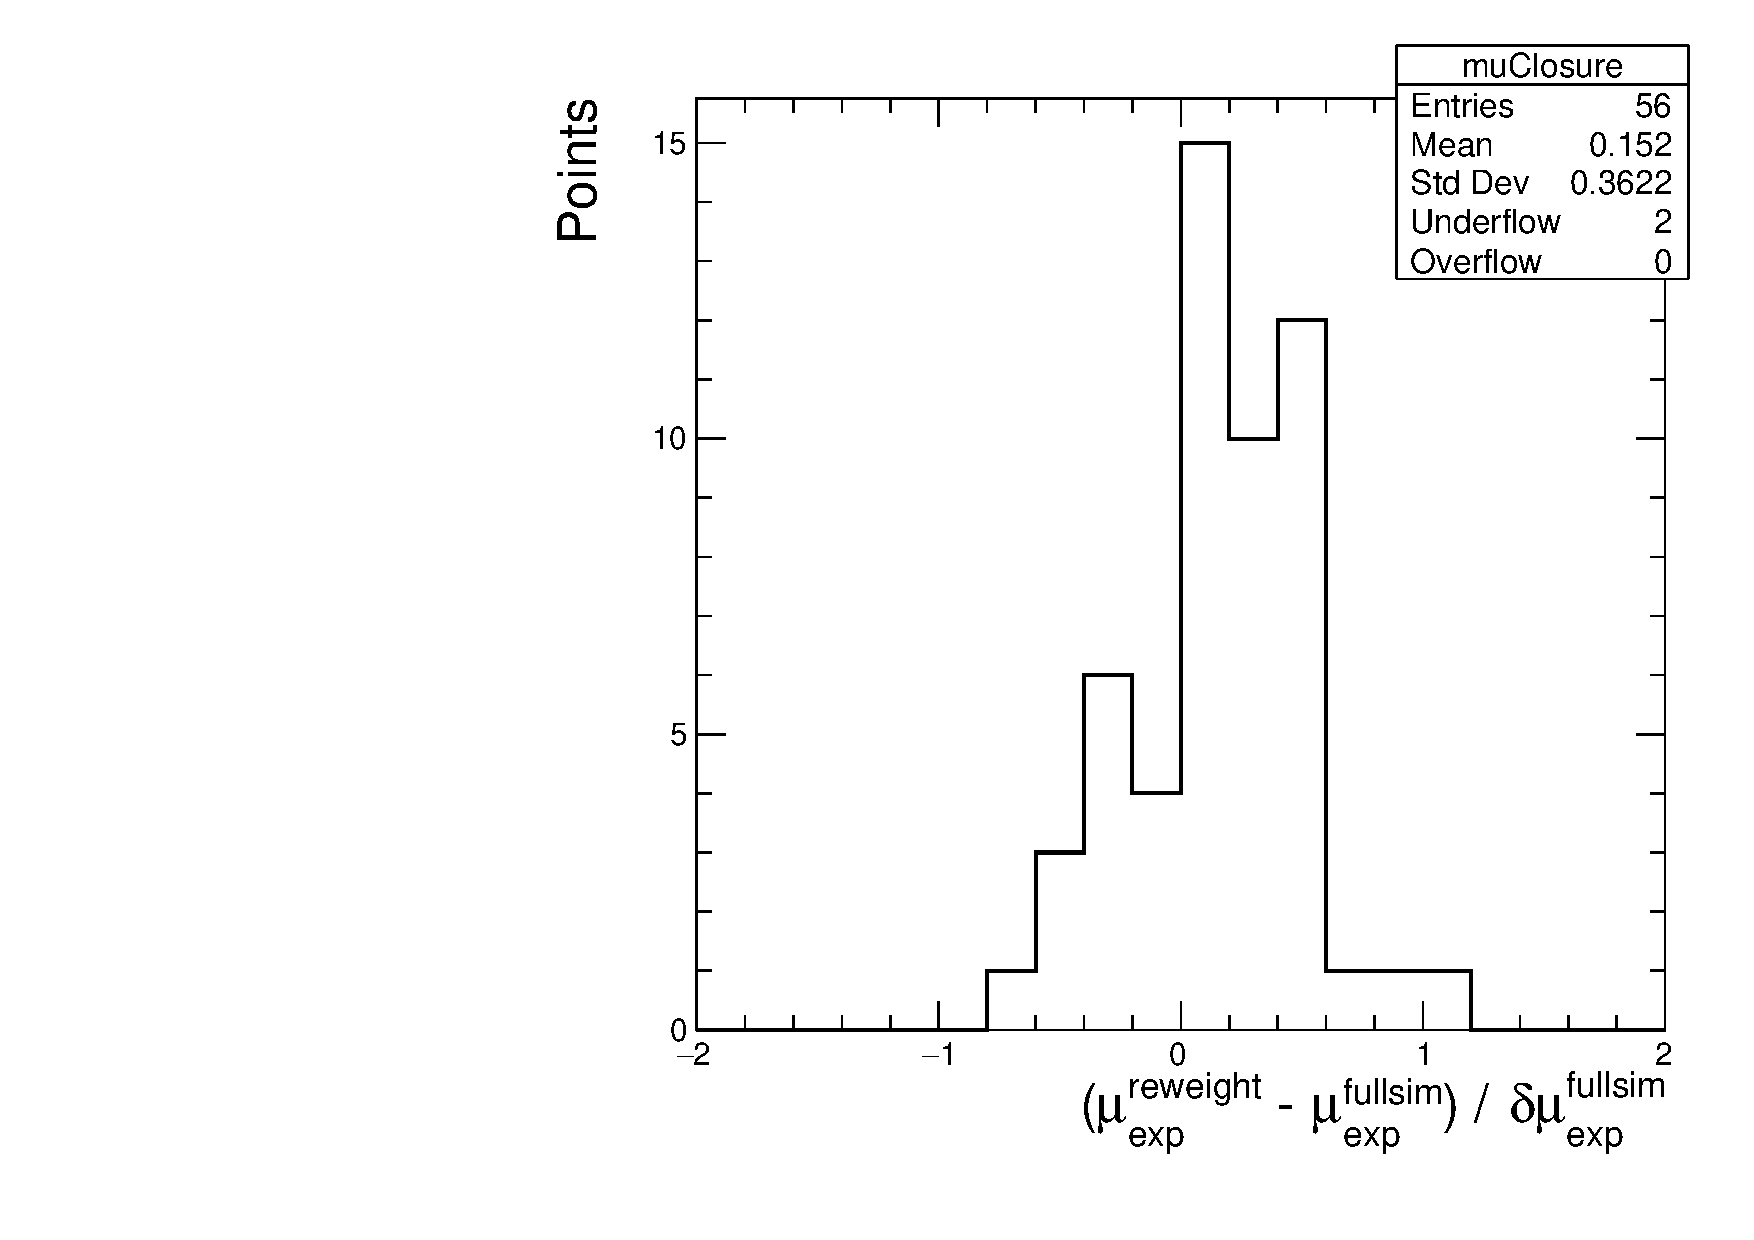
\includegraphics[width=0.48\textwidth]{figures/interpolation_appendix/reweightClosure_deltaMu.pdf}
     \caption{Closure test of final limits, showing change in the median expected signal strength ($\mu_{\rm exp} = \sigma_{\rm exp}/\sigma_{\rm theo}$) introducted by using the reweighting method for all points that have full simulation available.  The two underflow entries are the points $m_{A}=10, m_{\chi}=1$ and $m_{V}=10, m_{\chi}=1$. }
     \label{fig:app_interp_mu_pulls}
   \end{center}
 \end{figure}
 %-----------------------------------------------------



